%%%%%%%%%%%%%%%%%%%%%%%%%%%%%%%%%%%%%%%%%
% Thin Sectioned Essay
% LaTeX Template
% Version 1.0 (3/8/13)
%
% This template has been downloaded from:
% http://www.LaTeXTemplates.com
%
% Original Author:
% Nicolas Diaz (nsdiaz@uc.cl) with extensive modifications by:
% Vel (vel@latextemplates.com)
%
% License:
% CC BY-NC-SA 3.0 (http://creativecommons.org/licenses/by-nc-sa/3.0/)
%
%%%%%%%%%%%%%%%%%%%%%%%%%%%%%%%%%%%%%%%%%

%----------------------------------------------------------------------------------------
%	PACKAGES AND OTHER DOCUMENT CONFIGURATIONS
%----------------------------------------------------------------------------------------


\documentclass[11pt, french]{article}
\usepackage[french]{babel}
\selectlanguage{french}
\usepackage[T1]{fontenc}
\usepackage[utf8]{inputenc}
\usepackage{graphicx}
\usepackage{subcaption}
\usepackage[section]{placeins}

\usepackage[protrusion=true,expansion=true]{microtype} % Better typography
\usepackage{graphicx} % Required for including pictures
\usepackage{wrapfig} % Allows in-line images
\usepackage{float}
\usepackage{url}
\usepackage{mathpazo} % Use the Palatino font
\usepackage[T1]{fontenc} % Required for accented characters
\linespread{1.05} % Change line spacing here, Palatino benefits from a slight increase by default
\usepackage[french]{babel}
\selectlanguage{french}
\makeatletter
\renewcommand\@biblabel[1]{\textbf{#1.}} % Change the square brackets for each bibliography item from '[1]' to '1.'
\renewcommand{\@listI}{\itemsep=0pt} % Reduce the space between items in the itemize and enumerate environments and the bibliography

\renewcommand{\maketitle}{ % Customize the title - do not edit title and author name here, see the TITLE block below
\begin{flushright} % Right align
{\LARGE\@title} % Increase the font size of the title

\vspace{30pt} % Some vertical space between the title and author name

{\large\@author} % Author name
\\\@date % Date

\vspace{30pt} % Some vertical space between the author block and abstract
\end{flushright}
}

%----------------------------------------------------------------------------------------
%	TITLE
%----------------------------------------------------------------------------------------

\title{\textbf{Projet d'analyse d'image }\\ % Title
Détection et reconnaissance de panneaux de signalisation routière} % Subtitle

\author{\textsc{ Carlos Valadares , Gabriella Bettonte} % Author
\\{\textit{}}} % Institution

\date{\today} % Date

%----------------------------------------------------------------------------------------

\begin{document}

\maketitle % Print the title section


%----------------------------------------------------------------------------------------
%	ESSAY BODY
%----------------------------------------------------------------------------------------

\section{Introduction}

Ce projet s'inscrit dans le domaine d'étude du guide automatique: il vise à reconnaître automatiquement les panneaux de signalisation avec précision sans utiliser de techniques d’apprentissage automatique, en appliquant les connaissances théoriques acquises dans les cours de traitement d’images.\\

Diverses images contenant des panneaux de signalisation ont été fournies comme dataset. Les photos ont été prises à différentes distances, avec différentes illuminations et cameras pour simuler des situations pouvant se produire dans la réalité (regarder la figure \ref{fig:roads}). Il faut que notre application soit capable de détecter tous les signaux, qu'ils soient tournés, mal éclairés, lointains sans obtenir beaucoup de faux positifs, pour augmenter l'efficacité et le bon fonctionnement du système.\\

Pour le développement de l'application, on a utilisé Matlab.\\



\begin{figure}[h]
    \centering
    \begin{subfigure}[b]{0.4\textwidth}
        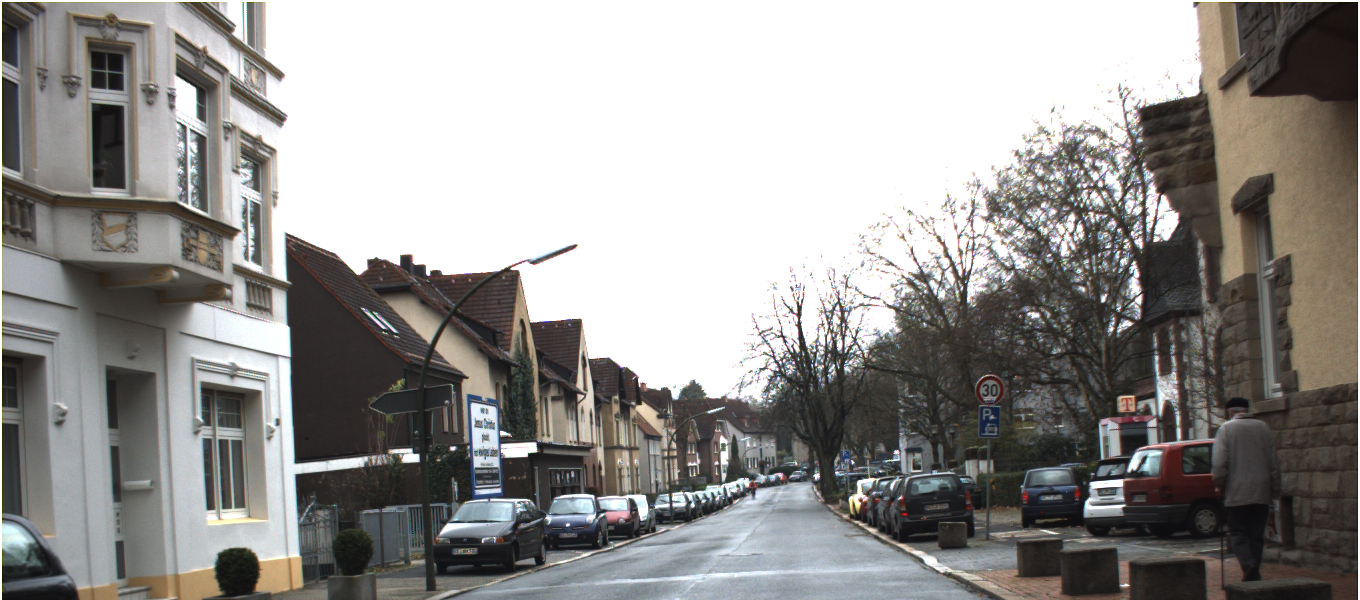
\includegraphics[width=\textwidth]{0.png}
        \caption{}
        \label{fig:0}
    \end{subfigure}
    ~ %add desired spacing between images, e. g. ~, \quad, \qquad, \hfill etc. 
      %(or a blank line to force the subfigure onto a new line)
    \begin{subfigure}[b]{0.4\textwidth}
        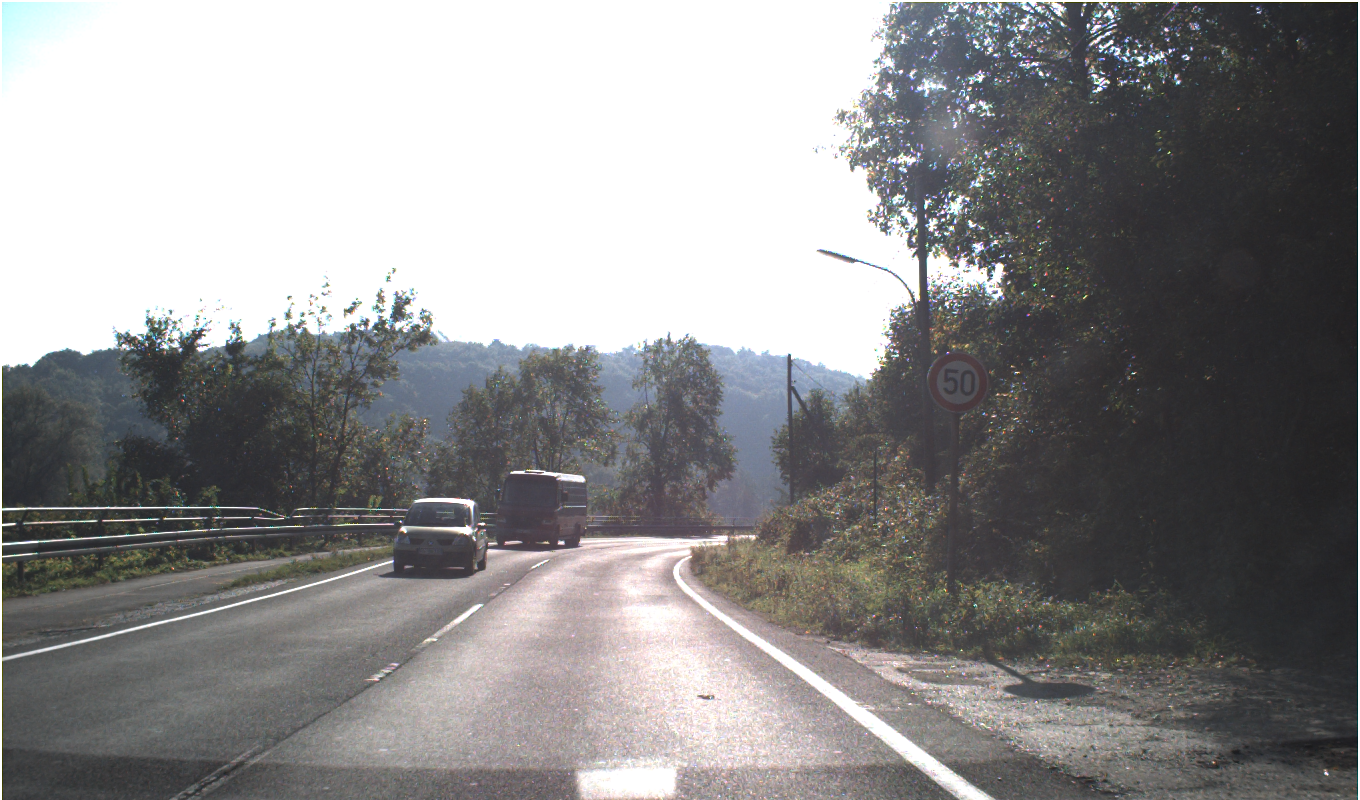
\includegraphics[width=\textwidth]{1.png}
        \caption{}
        \label{fig:1}
    \end{subfigure}
    \newline
    ~ %add desired spacing between images, e. g. ~, \quad, \qquad, \hfill etc. 
    %(or a blank line to force the subfigure onto a new line)
    \begin{subfigure}[b]{0.4\textwidth}
        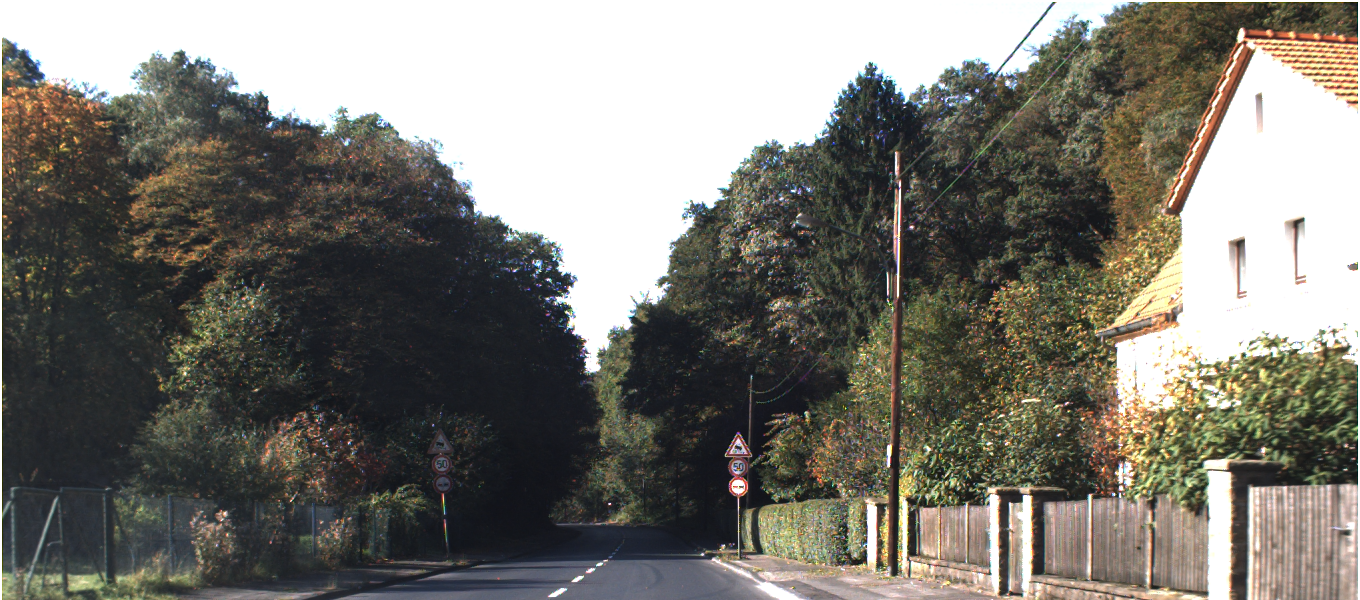
\includegraphics[width=\textwidth]{11.png}
        \caption{}
        \label{fig:11}
    \end{subfigure}
     \begin{subfigure}[b]{0.4\textwidth}
        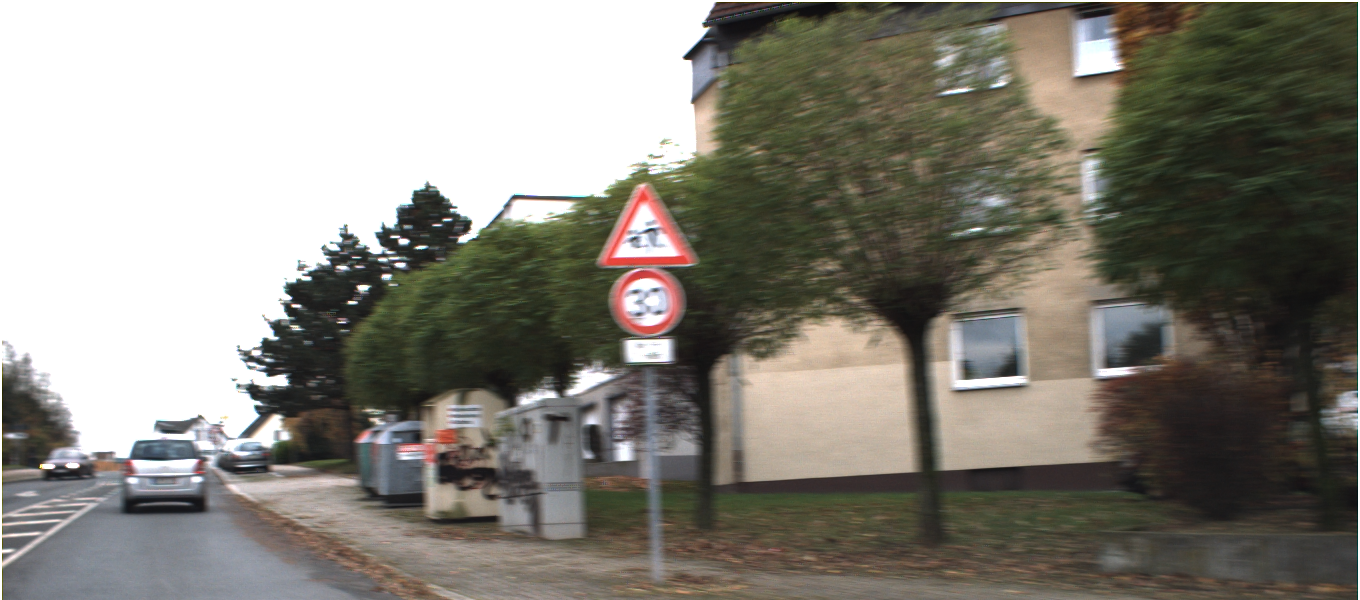
\includegraphics[width=\textwidth]{30.png}
        \caption{}
        \label{fig:30}
    \end{subfigure}
    \caption{Pictures of roads}\label{fig:roads}
\end{figure}

%------------------------------------------------
\section{Procédure}
\subsection{Coupage }
Après avoir observé les images, on a constaté que les panneaux de signalisation se trouvaient toujours dans la partie supérieure de l’image. On a donc décidé de couper les images à une hauteur égale au $\frac{3}{4}$ de la hauteur de l’image, fig.\ref{fig:taglio}.\\
Cette opération nous a semblé légitime car, puisque nous sommes dans le domaine de la conduite automatique, il est plausible que les panneaux de signalisation à reconnaître, pendant que la voiture roule, se situent dans la partie supérieure de la vue et non à proximité du sol.\\

\begin{figure}[h]
    \centering
    \begin{subfigure}[b]{0.4\textwidth}
        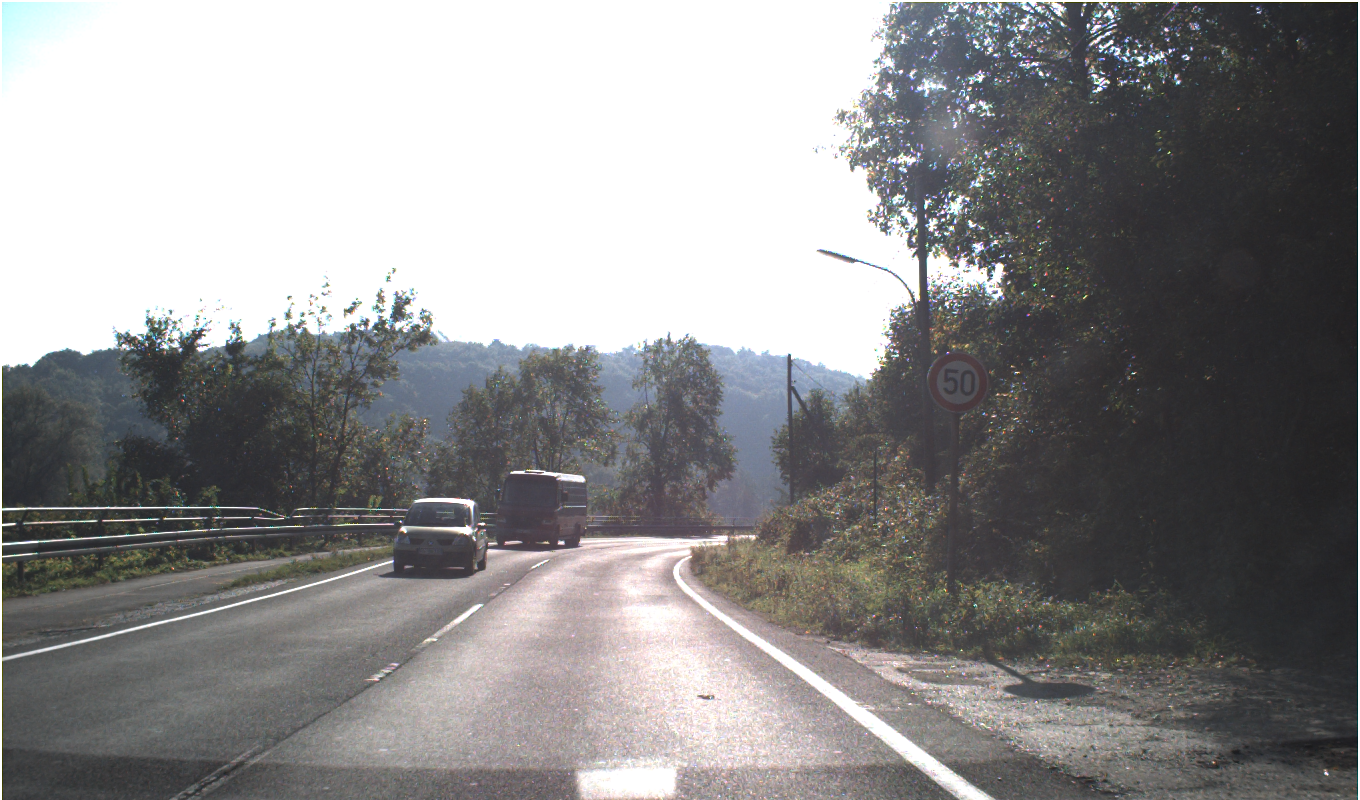
\includegraphics[width=\textwidth]{1.png}
        \caption{}
        \label{fig:1}
    \end{subfigure}
    ~ %add desired spacing between images, e. g. ~, \quad, \qquad, \hfill etc. 
      %(or a blank line to force the subfigure onto a new line)
    \begin{subfigure}[b]{0.4\textwidth}
        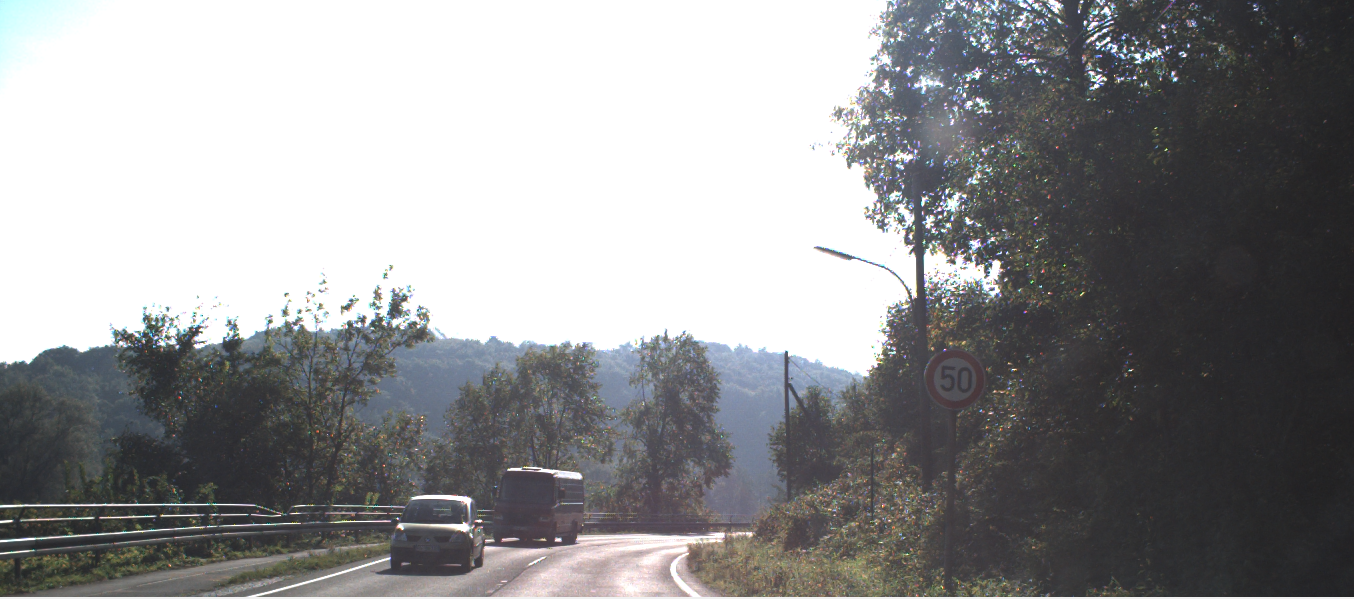
\includegraphics[width=\textwidth]{tag1.png}
        \caption{}
        \label{fig:tag1}
    \end{subfigure}
    
    
    \caption{Coupage à une hauture de $\frac{3}{4}$}\label{fig:taglio}
\end{figure}
 
\subsection{Normalisation} 
Ensuite, on a transformé l'image RGB en une image RGB normalisée. Pour cela, nous avons écrit la fonction matlab \textit{RGBNormalize} qui a pour paramètre d'entrée l'image originale et qui renvoie l'image normalisée.\\
Au début, nous avions simplement essayé de diviser chaque canal de couleur par $255$, mais cette idée a donné de mauvais résultats.\\
Nous avons donc constaté que la normalisation donnant de bons résultats est la suivante:
$ \left( \frac{R}{\sqrt{R^2+G^2+B^2}}, \frac{G}{\sqrt{R^2+G^2+B^2}} , \frac{B}{\sqrt{R^2+G^2+B^2}} \right)$.



On peut appeler cela une normalisation car la somme de ces trois factions donne 1.\\



\begin{figure}[h]
    \centering
   
        
\includegraphics[width=\textwidth]{norma.png}
        \caption{}
        \label{fig:norma}
   
   
    
    
    
    \caption{Normalisation}
\end{figure}

\subsection{Seuillage } 
En suite, on a analysé l'image avec l'aide de le curseur matlab et on a choisi les bonnes seuils à la main:\\
\begin{itemize}
\item $RMeanTreshold = 0.63$;
\item $GMeanTreshold = 0.55$; 
\item $BMeanTreshold = 0.6$.

\end{itemize}
\bigskip
On a sélectionné dans l'image les zones contenant une valeur rouge supérieure à \textit{RMeanTreshold} et les valeurs bleue et verte ci-dessous à \textit{BMeanTreshold} et \textit{GMeanTreshold} 
\subsection{TO BE FIXED: } 


Ici, je ne me souviens pas bien parce que nous avons fait BWAREAOPEN et comment nous avons extrait le fonds.
apres on a fait le canny: il faut expliquer

+IMAGE FOND


\subsection{Post-traitement }
Après avoir sélectionné les contours de l'image, comme expliqué au point précédent, on s'est consacré à la réalisation d'un post-traitement pour améliorer la détection des panneaux de signalisation.\\
Nous avons réalisé une expansion avec un élément structurant de disque afin de fermer les contours pour délimiter parfaitement la zone souhaitée.

FILLED POUR REMPLIR LE TROUS+ IMAGE

\subsection{ bounding box }

BOUNDING BOX ET EXPLIQUER LE CONDITIONES.+IMAGE


\textbf{----------------------------------------------------------------------}\\

TO BE FIXED: 
\section{blabla}
HSV:
\begin{itemize}
\item porquoi hsv
\item comme
\end{itemize}
probleme: Problem avec thresholding 
solution: color segmentation app

problem : plaque loin ou peu illumine
solution: RGB normalized (pour avoir plus de performance)

\section{idee future}
\begin{itemize}
\item esseyer avec filtre gaussian avant segmentation
\item S entre 0.2-0.5
\item overture
\item bwareaopen
\end{itemize}

NB pas obligé de faire un segmentation perfaite

\section{TP 11 janvier}

\begin{itemize}
\item nous avons essayé de calculer la luminosité avec cette formule $ Y=0.2126R+0.7152G+0.0722B$ 
mais dans les images normalisées, il y avait toujours la même valeur $0.3333$\\

au lieu de cela, dans les images, rgb n'était pas une donnée utile car nous ne pouvions pas détecter de motif parmi les images mal détectées

\item 

\end{itemize}

après ona fait image original- bwareaopen()

img.23--> probleme de detection\\
img.16--> il a beaucoup de pixels\\
toutes le autres pas detectés: probleme de connexité

\section{future pt.2}

on va essayer de faire une ouverture pour éliminer le petits choses.






\section{Etapes principales}

\subsection{Seuillage}
dffhiufdhf\\

porquoi et comment\\

Problems\\

Solution\\


\subsection{Detection}

\subsection{Classification}

\section{Conclusion}

\subsection{Retrospective}

\subsection{Idées futures}






\newpage
\begin{thebibliography}{99}

\bibitem{canny} OpenCV Canny's tutorial \url{https://docs.opencv.org/3.4/da/d5c/tutorial_canny_detector.html}

\end{thebibliography}


%----------------------------------------------------------------------------------------

\end{document}